\clearpage{\pagestyle{empty}\cleardoublepage}

\chapter{The ATLAS experiment at the Large Hadron Collider}\label{chap:atlas}

The analyses presented in this dissertation have been performed analyzing data from 
proton-proton (p-p) collisions at the \cme $\rts=8\tev$ recorded during the year 2012 
at the ATLAS experiment~\cite{Aad:2008zzm}. In the following Chapter we will briefly 
describe the main features of the detector, located at the CERN laboratories in Geneva,
Switzerland.

The experimental facilities are situated at Point~1 along the Large Hadron Collider 
(LHC)~\cite{lhc} 27~km long ring, shown in Figure~\ref{fig:lhcring}. The accelerator
tunnel can reach an underground depth of 175~meters and is spread between Swiss
and French territory, while the cave where ATLAS is allocated is about 100~meters 
underground in the CERN Swiss site of Meyrin. 

\begin{figure}[tb]\begin{center}
	\subfigure{\label{fig:lhcring}
  	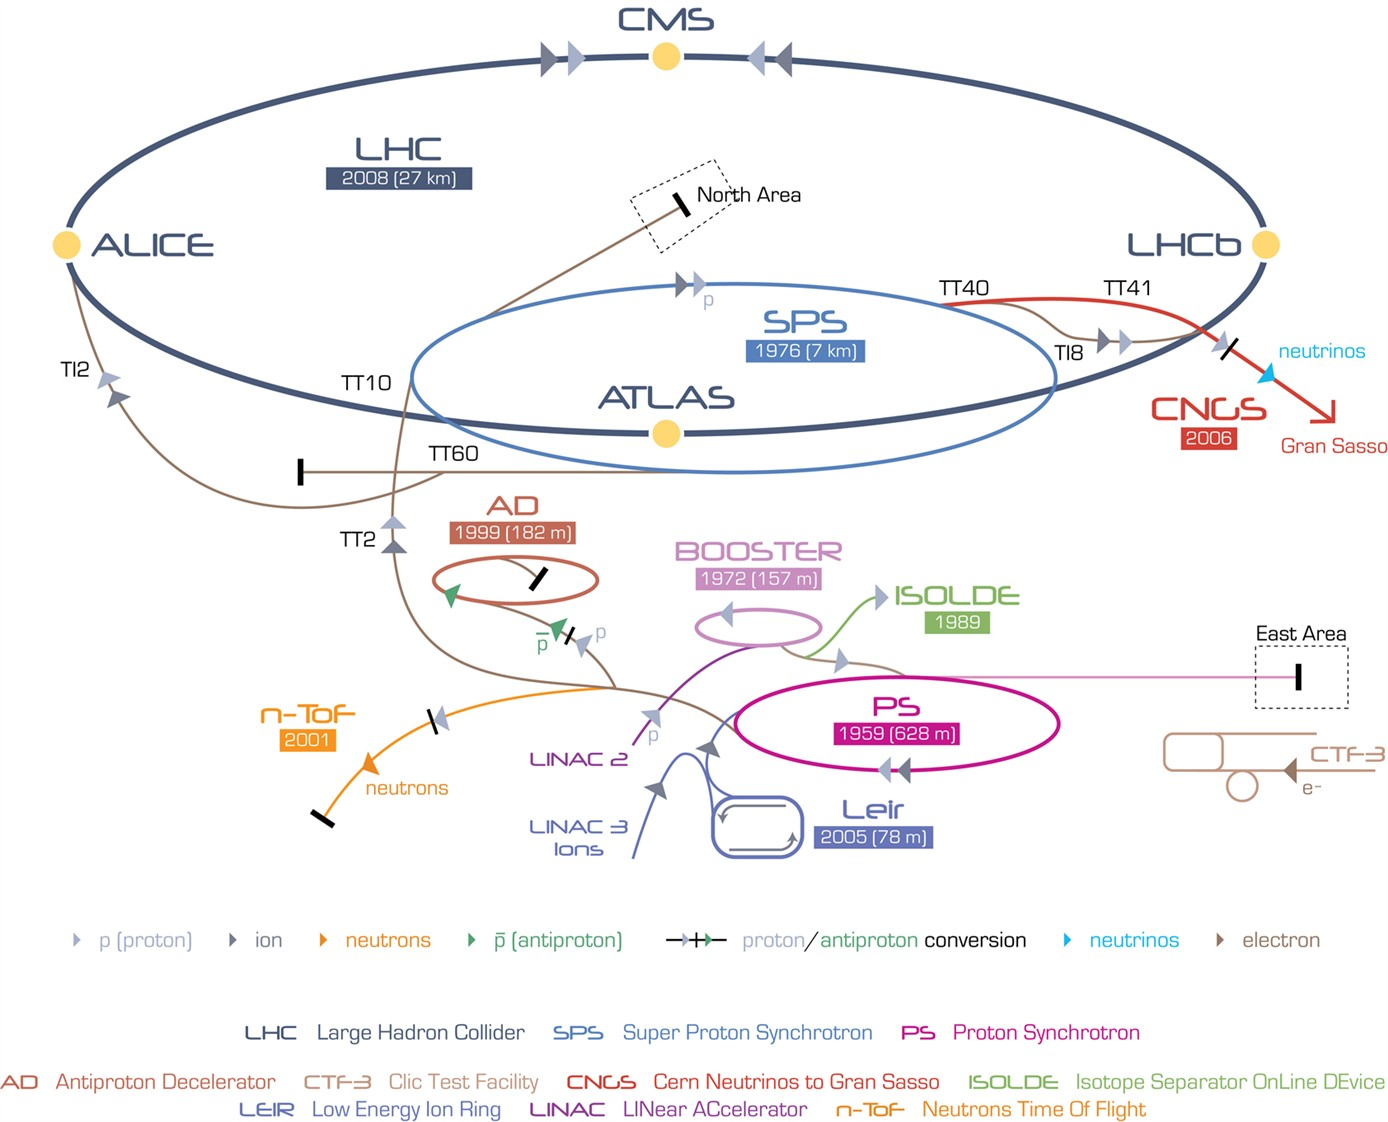
\includegraphics[width=0.8\textwidth]{detector/figures/ring.eps}}
	\caption{A schematic showing the accelerator complex at CERN. Protons are
        extracted from Hydrogen gas and injected in the first machine, the linear 
        accelerator LINAC2 that starts the acceleration chain. When protons reach
        an energy of 50\mev they are injected into the Proton Synchrotron Booster
        (PSB) and accelerated up to the energy of 1.4\gev. The second circular
        accelerator, the Proton Synchrotron (PS) brings the energy of the protons
        to 25\gev previous to injecting them into the last machine before the LHC,
        the Super Proton Synchrotron (SPS). Protons of 450\gev finally enter the
        LHC where they are boosted to energies of up to 4\tev.
        The four main LHC experiments are shown on the collider ring.}
\end{center}\end{figure}

The LHC program was approved by CERN Council in 1994, followed by the approval of
the four main experiments physics programs: ATLAS~\cite{Aad:2008zzm} and CMS~\cite{cms}
in 1996; ALICE~\cite{alice} in 1997; LHCb~\cite{lhcb} in 1998.
Works towards the installation of the most powerful particle accelerator of the world
started when the Large Electron Positron Collider (LEP) was dismantled in 2000 to 
give up its place in the tunnel to the LHC, which was then fully operational by 2008.

The LHC is composed of eight arcs 2.7~km long, each of which contains 154 dipole 
magnets, whose function is to  bend the beams along the circular trajectory, and
49 quadrupole magnets, that focus the beam. These superconducting magnets operate
at a temperature of 1.9~K, maintained by means of liquid Helium vessels.
Eight insertions are placed inbetween the arches. Each insertion has a specific
role that characterizes its design and can be injection, beam dumping, beam cleaning,
or ``physics'', i.e. make the beams collide within an experiment.

First proton beams were circulated on 10th September 2008 and right on the verge of
getting the first collisions at a \cme $\rts=900\gev$ nine days later, an electrical
connection joining superconducting wires of a dipole and a quadrupole
failed. This caused the release of liquid Helium in the insulating vacuum,
resulting in an explosion that severely damaged the machine.
After more than one year devoted to repair the damage and consolidate the security,
on 30th November 2009 the LHC became the world's highest energy particle 
accelerator\footnote{\url{http://press.web.cern.ch/press/PressReleases/Releases2009/PR18.09E.html}}:
\begin{quotation}\small
Geneva, 30 November 2009. CERN's Large Hadron Collider has today become the world’s highest energy particle accelerator, having accelerated its twin beams of protons to an energy of 1.18 TeV in the early hours of the morning. This exceeds the previous world record of 0.98 TeV, which had been held by the US Fermi National Accelerator Laboratory’s Tevatron collider since 2001. It marks another important milestone on the road to first physics at the LHC in 2010.
\end{quotation}





The main performance figure of merit for an accelerator is the luminosity, the 
instantaneous luminosity $\mathcal L$ being defined as 
\begin{equation}\label{eq:lumiN}
\mathcal{L}\times\sigma=\dfrac{dN}{dt}=f\times n\dfrac{N_1\times N_2}{A}\times\sigma.
\end{equation} 
Here $dN/dt $ is the event rate of a certain process and $\sigma$ is its cross 
section. This rate is directly proportional to the the frequency $f$, the number 
of bunches $n$ and the number of particles in the two bunches $N_1, N_2$, and
inversely proportional to the beam cross-section $A$.

Integrating over the accelerator active time (a ``fill'', when stable beams are kept
colliding) gives the \textit{integrated luminosity}, relating the total number 
of produced events $N_{tot}$ to the cross-section:
\begin{equation}\label{eq:intLumi}
\int \mathcal L dt  = \dfrac{N_{tot}}{\sigma} 
\end{equation}
